\section{Tandem Affinity Purification (TAP)}\footnote{\url{https://en.wikipedia.org/wiki/Tandem_affinity_purification}}

\textbf{Verwendung:} Welche Proteine interagieren untereinander? Suche nach einzelnen Proteinen und Proteinkomplexen\\

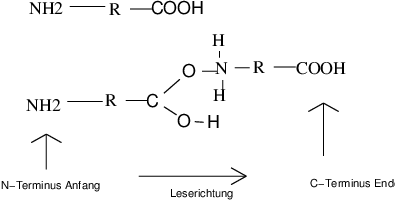
\includegraphics[width=0.75\textwidth]{lectures/160513/pix/namenlos.png}

\underline{TAP-Tag}\\
 - C-terminal variante (es gibt auch n-terminal)

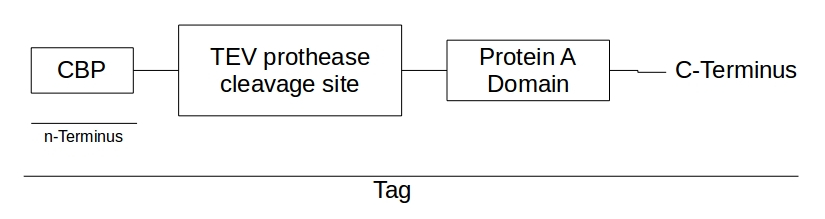
\includegraphics[width=0.75\textwidth]{lectures/160513/pix/1.jpg}
\\\\
CBP - Calmodulin binding peptide\footnote{\url{https://en.wikipedia.org/wiki/Calmodulin}}\\
TEV - tabacco etch virus\footnote{\url{https://en.wikipedia.org/wiki/Tobacco_etch_virus}}\\
IgG - unspezifischer Antikörper (Immunglobulin G)\footnote{\url{https://de.wikipedia.org/wiki/Immunglobulin_G}}
\\\\
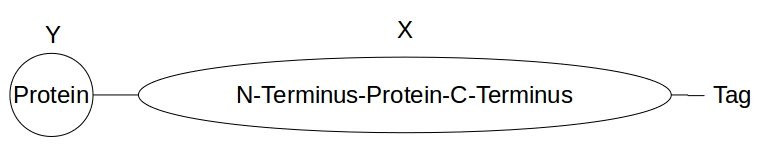
\includegraphics[width=0.75\textwidth]{lectures/160513/pix/2.jpg}
\\\\
\textbf{Protein Y wird gesucht!} (Tag wird in Plasmid eingeschleußt)

\begin{enumerate}
	\item Plasmid mit getaggtem Protein \& Interaktionspartner werden in Hefezellen inkubiert
	\item Affinity purification (Ähnlichkeit Aufreinigung): IgG Matrix bindet die Protein A Domain des Tags (am Ende bleint Tag übrig)
	\item mit Hilfe der TEV protease um an TEV protease cleaveage site zu schneiden
	\item Calmodium beads um Protein zu extrahieren
	\item Auftrennen der Proteine, z.B. durch Ultraschall (nur Interaktionsbindung, keine Peptidbindung!)
	\item Indentivizieren von Y durch Massenspektrometer
\end{enumerate}

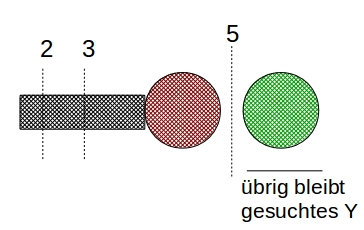
\includegraphics[width=0.5\textwidth]{lectures/160513/pix/3.jpg}

\textbf{Probleme:}
\begin{itemize}
	\item durch (häufige) Reinigung hohe Fehlerrate
	\item durch Tag an Protein Faltung möglicherweise nicht mehr (wie ursprünglich) möglich
\end{itemize}

\underline{weitere Informationsquellen (indirekt)}\\\\
Ziel: Reduzierung des False-Negatives
\begin{itemize}
	\item Interaktion über Protein-Protein-Bindungsdomain: Vorhersage über Markovmodelle möglich (Domain, Interaktionspartner)
	\item Homologie: Vorhersage über Interaktionen in nahen Verwandten
	\item Textmining auf Publikationen
\end{itemize}

\underline{Filterung}\\\\
Ziel: Reduzierung der False-Positives
\begin{itemize}
	\item Co-Expression: werden 2 Proteine gleichzeitig expremiert?
	\item Lokalisationsinformationen: wenn nicht im gleichen Kompartiment vorhanden, Interaktion nicht möglich
\end{itemize}

$\Rightarrow$ Ergebnisse durch vorherige Vorgänge: Protein-Protein-Interaktionsnetzwerke in einer Spezies\\
\textbf{$\Rightarrow$ Analyse des Netzwerks}
\\\\
Protein-Protein-Interaktionsnetzwerk (PPIN) = Graph G = (V,E)\\
V = Knoten (Proteine)\\
E = Kanten (Interaktionen) $\subseteq$ VxV $\rightarrow$ erzeugt Paare von Konten\\
$\rightarrow$ ungerichtete Graphen: (a,b) $\in$ E $\Leftrightarrow$ (b,a) $\in$ E

\subsection{Local clique merging algorithm (LCMA)}
clique - vollständige subgraphen C\\
$C=(V',E')$ mit $V'\subseteq V$, $E'\subseteq E$\\
$\forall x,y \in V': (x,y) \in E'$\\
\\
Annahme: dichte Subgraphen repräsentieren Proteinkomplexe\\\\
Dichte von G: $\delta(G) = {2 \cdot |E| \over |V| \cdot |V-1|}$\\

\underline{Suche nach dichten Graphen}
\begin{enumerate}
	\item Suchen Knoten u in G mit dem kleinsten Grad (Grad eines Konten = Anzahl der Kanten die von einem Knoten ausgehen)
	\item entfernen Knoten (+ Kanten) mit dem geringsten Grad $\Rightarrow$ erhöht die Dichte in Graphen: $G'=G\backslash\{u\}$
	\item wiederhole ab 1 solange gilt: $\delta(G') > \delta(G)$
\end{enumerate}

$\Rightarrow$ lokale Cliquen $C_{1},…,C_{n}$\\\\
\underline{Merge:}\\
Overlap von $C_{x}=(V_{x},E_{x})$ \& $C_{y}=(V_{y},E_{y})$\\
\begin{equation}
Overlap={|V_{x} \cap V_{y}|^2 \over |V_{x}| \cdot |V_{y}|}
\end{equation}
wenn Overlap $>$ cut-off $C_{x} \cup C_{y}= (V_{x} \cap V_{y}, E_{x} \cap E_{y})$\\\\
Solange wie noch Cliquen gemerged werden \& $\underbrace{\sum \limits_{n} \frac{\delta(n)}{N}}_{average density}$ nicht signifikant schlechter wird (AD' $>$ 0,95 AD)\\\\
$\rightarrow$ Verleich mit realen Proteinkomplexen hat gezeigt, das Cliquen keine gute Approximation ergeben

\subsection{Clique Finding Algorithzm (CFA)}
Annahme: Proteinkomplexe k-connected\footnote{\url{https://de.wikipedia.org/wiki/K-Zusammenhang}}\\
graphs $\Rightarrow$ geringe Dichte möglich\\
k-connected: $k \in \mathbb{N}$ $\forall V' \subset V, |V'| < k$, G zusammenhängend\\
k $\rightarrow$ Anzahl der Knoten, die entfernt werden können, ohne das G auseinanderfällt\\
$\Rightarrow$ alle Knoten haben Grad $>$ k
\\\\
\begin{enumerate}
	\item entferne alle Knoten mit Grad $<$ k
	\item wenn der resultierende Graph weniger als k Knoten hat $\rightarrow$ kein k-connected Subgraph
	\item finden \{$u_{1},…,u_{n}$\}, n$<$k, so dass $G\backslash \{u_{1},…,u_{n}\}$ nicht mehr zusammenhängen, es entstehen Zusammenhangskomponenten
\end{enumerate}

$\Rightarrow$ für jede Zusammenhangskomponente beginnen bei 1.\\
wenn {$u_{1},…,u_{n}$\} nicht existiert $\Rightarrow$ G ist k-connected
\newpage
\underline{Beispiel:} k=2
\begin{center}
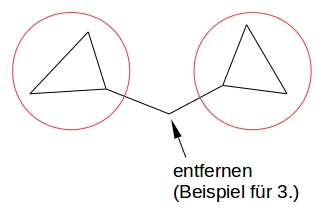
\includegraphics[width=0.5\textwidth]{lectures/160513/pix/5.jpg}
\end{center}

k $\Rightarrow$ Suche Anzahl n $<$ k = Anzahl der Knoten die entfernt werden können ohne dass der Graph auseinanderfällt
\begin{itemize}
	\item 1-connected
	\item 2-connected
	\item …
	\item n-connected
\end{itemize}

Filtern: dia(G) = Durchmesser von G (Länge des längsten Pfades)\\
k=1 $\Rightarrow$ dia(G) = 4\\
k=2 $\Rightarrow$ dia(G) $>$ 2$\cdot$k\\
rausgefiltert werden alle dia(G) $<$ 2$\cdot$k, da dort die Dichte hoch